\chapter{Теоретический раздел}

\section{Цель работы}
Целью данной лабораторной работы является изучение методов классификации изображений с помощью нейронных сетей на примере датасета MNIST, а также исследование влияния архитектуры сети и соотношения обучающей и тестовой выборок на качество обучения.  

\section{Задачи работы}
\begin{enumerate}
    \item Создать нейронные сети с различным количеством скрытых слоев (0, 1, 5) с использованием активации ReLU и функции потерь KL Divergence.
    \item Обучить сети на различных долях обучающей выборки (10\%, 20\%, ..., 90\%) и оценить точность на обучающей и тестовой выборках.
    \item Определить состояния переобучения и недообучения.
    \item Рассчитать минимальный размер обучающей выборки с помощью неравенства Чебышёва.
\end{enumerate}

\section{Нейронные сети и функции активации}

Нейронная сеть представляет собой последовательность слоёв, каждый из которых выполняет линейное преобразование и нелинейную активацию.  
Для скрытых слоёв использовалась активация ReLU (\textit{англ. Rectified Linear Unit}), график которой представлен на рисунке \ref{relu}:
\begin{equation}
    f(x) = \max(0, x)
\end{equation}


На выходном слое применялся LogSoftmax для использования с функцией потерь KL Divergence:
\begin{equation}
    \text{LogSoftmax}(z_i) = \log \frac{e^{z_i}}{\sum_{j} e^{z_j}}
\end{equation}

Функция потерь KL Divergence между предсказанным распределением $q$ и истинным распределением $p$ записывается как:
\begin{equation}
    D_{KL}(p \parallel q) = \sum_{i} p_i \log \frac{p_i}{q_i}
\end{equation}

\begin{figure}[h]
\centering
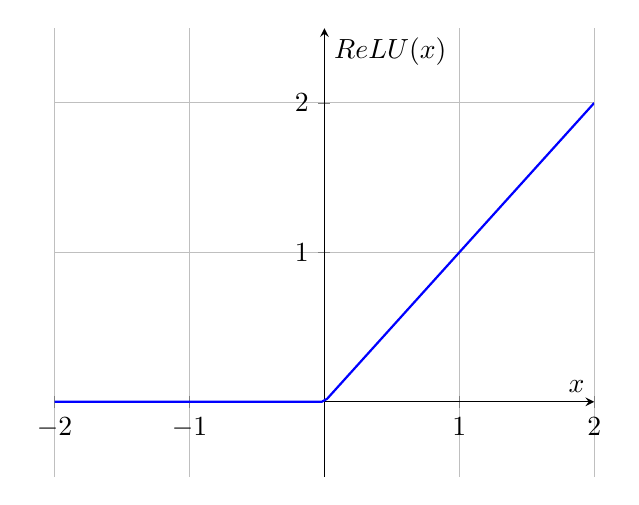
\begin{tikzpicture}
\begin{axis}[
axis lines = middle,
xlabel = $x$,
ylabel = {$\text{ReLU}(x)$},
xmin=-2, xmax=2,
ymin=-0.5, ymax=2.5,
samples=100,
domain=-2:2,
grid=both,
]
\addplot[blue, thick] {max(0,x)};
\end{axis}
\end{tikzpicture}
\caption{График функции ReLU}
\label{relu}
\end{figure}

\section{Неравенство Чебышева для оценки минимального размера выборки}

Для случайной величины $X$ с математическим ожиданием $\mu$ и дисперсией $\sigma^2$ справедливо неравенство Чебышева:
\begin{equation}
    P(|\bar{X} - \mu| \ge \epsilon) \le \frac{\sigma^2}{N \epsilon^2}
\end{equation}
где $\bar{X}$ --- среднее по $N$ наблюдениям, $\epsilon$ --- допустимая ошибка.  

При оценке минимального размера обучающей выборки для задачи классификации удобно использовать дисперсию Бернулли:

\begin{equation}
\sigma^2 = p (1 - p)
\end{equation}

где
    $p$ — ожидаемая точность модели на выборке;  
    $(1-p)$ — вероятность ошибки классификации.

Тогда неравенство Чебышева примет вид:

\begin{equation}
P(|\bar{X} - p| \ge \epsilon) \le \frac{p (1 - p)}{N \epsilon^2}
\end{equation}

Из него выводим минимальный размер выборки:

\begin{equation}
N \ge \frac{p (1 - p)}{\delta \, \epsilon^2}
\end{equation}

где $\delta = 1 - P$ — вероятность того, что отклонение превысит $\epsilon$.


% \includeimage
%     {tux} % Имя файла без расширения (файл должен быть расположен в директории inc/img/)
%     {f} % Обтекание (без обтекания)
%     {h} % Положение рисунка (см. figure из пакета float)
%     {0.25\textwidth} % Ширина рисунка
%     {Символ Linux (Tux)} % Подпись рисунка

